\subsection{Auto-curriculum learning improves performance} \label{sec:results_curriculum}


To establish the importance of automated curriculum learning, we compare adaptation when training with the curricula methods outlined in Section~\ref{sec:methods_auto_curriculum}: no-op filtering and PLR. Figure~\ref{fig:curricula_performance} shows the median last-trial score of agents trained with different curricula. Both no-op filtering and PLR curricula strongly outperform a baseline trained with uniformly sampled tasks. Moreover, PLR outperforms No-op filtering, particularly at a higher number of trials, indicating that a regret-based curriculum is especially helpful for learning longer-term adaptation. In Appendix \ref{app:autocurriculum} we detail training configuration, and also compare the sample efficiency of our methods, where we see that both auto-curriculum approaches are more sample-efficient than uniform sampling, in terms of both learning steps and FLOPs.

\begin{figure}[htb!]
    \centering
    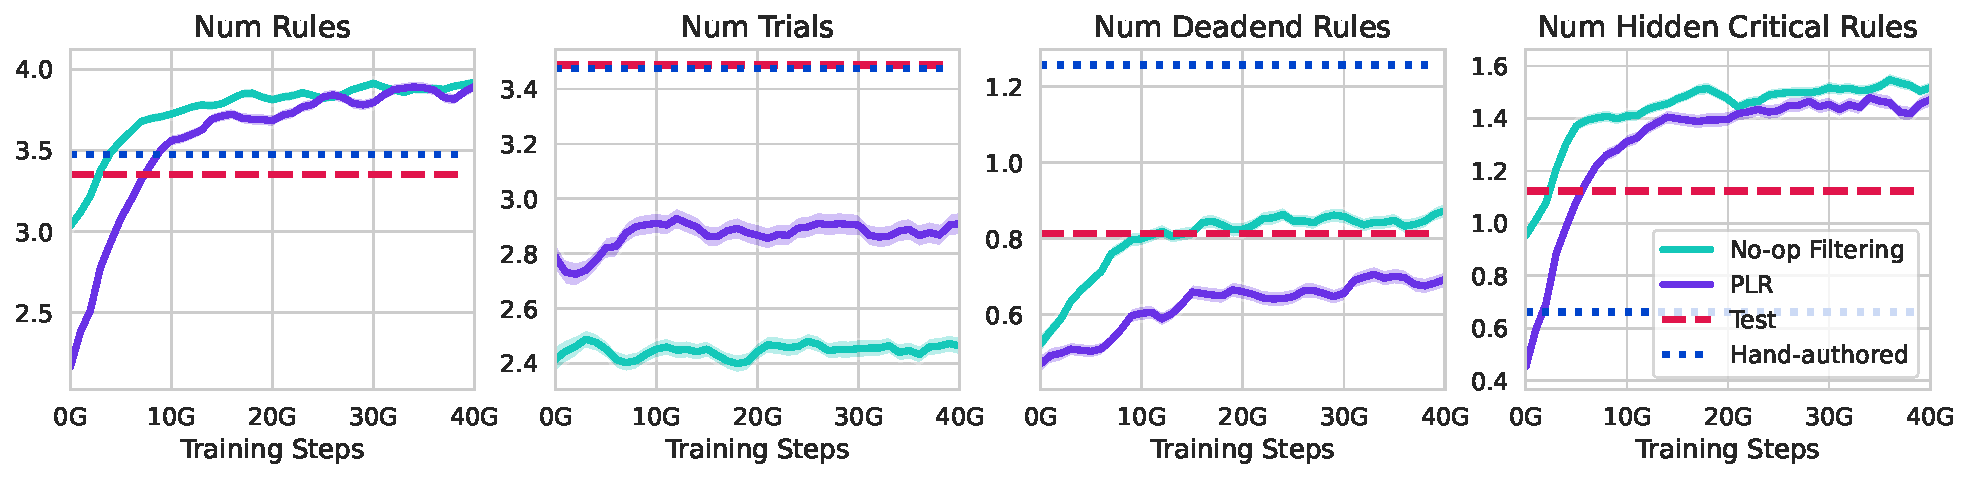
\includegraphics[width=0.99\linewidth]{figures/curriculum/emergent_curricula.pdf}
    \caption{
        Emergent curricula for no-op filtering and PLR. Plots show a selection of task metrics for the dynamic training set, averaged over all tasks in the set, with standard error shaded. In all plots, a higher metric value corresponds to greater task difficulty. For example, tasks with a higher number of rules require more trial-and-error to find the correct rules to trigger. Horizontal lines show the same metric values averaged over the test (dashed) and hand-authored (dotted) evaluation task sets.}
    \label{fig:emergent_curricula}
\end{figure}

In Figure~\ref{fig:emergent_curricula} we show the evolution of task complexity for both methods. In both cases, simpler tasks are initially prioritised, with a clear curriculum emerging. Neither method explicitly optimises to increase these metrics, yet the task complexity increases as a result of the agent's improving capabilities. See Figure~\ref{fig:emergent_curricula_extended} for additional metrics of task complexity.

